\documentclass[a4paper,11pt]{article}

\usepackage{float}
\usepackage{graphicx}
\setlength{\oddsidemargin}{0in}
\setlength{\evensidemargin}{0in}
\setlength{\textwidth}{160mm}
\setlength{\topmargin}{-15mm}
\setlength{\textheight}{240mm}

\graphicspath{./Diagrams}

\begin{document}

\section{Experiment methods}

\subsection{Experiment 1}
There are two distinct algorithms being used in this project, the Hybrid Repair and the Multi-objective algorithm. These two algorithms both have there strengths and weaknesses and whilst not the ideal choice for solving sudoku, one of these methods might be better than the other. So the question becomes: 
\begin{itemize} 
     \item How does a hybrid repair EA algorithm compare to a Multi-objective EA? 
     \item Is one method more efficient than the other?
     \item Is one method more consistent than the other?
     \item Is there a large difference in runtime?
\end{itemize}
The first question can be answered by looking at the next three questions. For finding out the efficiency or effectiveness of the algorithms, looking at and comparing the number of generations it takes to get to the solution.  For finding out the consistency of the algorithms, looking at the number of times each algorithm fails to solve the puzzle it is presented and also looking at the standard deviation from the average number of generations and runtime. \newline \newline The final question has the least impact on the overall investigation, as it can be affected the most by outside factors, however looking at the average runtimes and standard deviations from the average can clearly show how fast each algorithm generally, however it also worth noting, that this could be due to inefficient programming rather than the algorithms design itself. Due to the randomness of both of the algorithms, both sets of results will have to process and compared using a statistical test which can data that is not normally distributed such as a Wilcoxon test.
\subsection{Experiment 2}
The second and arguably more interesting question being looked at in this project, concerns difficulty in Sudoku puzzles. With Sudoku puzzles, there are two main ways to increase the difficulty of the puzzles, the first is by increasing the size of the puzzle, as with larger puzzles, there are more numbers involved and more potential solutions. Meaning that inherently a 4x4 puzzle is easier than a 9x9 puzzle. The other way in which difficulty can be measured for people, is by changing the number of initial squares that are filled. Concerning the minimum number of spaces required for a unique solution to be found by a human, research has been done and it has been found that a minimum of 17 filled in spaces are needed for a Sudoku to be solvable.\newline \newline For the purposes of this question broader catagories for difficulty, will be more appropriate, this will be done by using sudoku generated by Sudoku.com[] and using their difficulty system of Easy, Medium, Hard and Extreme puzzles. The interesting part comes from looking for a link between the difficulty that humans find solving these puzzles and the algorithms that are designed to do so. By looking at both algorithms and using them on different difficulty sets, some questions are created:
\begin{itemize}
	\item Is there a correlation between human difficulty and algorithm performance?
	\item Does either algorithm perform particularly well with a certain difficulty or size puzzle? Why?
	\item Is the relationship between initial puzzle size and generations?
\end{itemize}
For the first question, looking at a mapped graph displaying difficulty against runtime and generations. For the second question, looking at the results for the datasets on both sides for each difficulty and finding any noticable difference in the averages outside of the conclusions from experiment 1. The final question further builds on question 1, by seeing if the correlation is simply due to the size of the puzzle given.

\subsection{Approach for Hybrid Repair method}

The idea for the hybrid method is, firstly much like a normal EA the population of the puzzle is created , this will be generated from many starting mutations on the initial sudoku puzzle given. The next step is a loop, that if there are no violations and no empty spaces in any puzzle population, or alternatively the algorithm has reached the maximum number of generations, ends the loop and returns the solution if there is one, otherwise the rest of the steps are taken, all of which are contained within this loop. The next step is sorting and selection, this will take the population, sort them based on their fitness values and then removes half the puzzles from the population. The remaining members of the population would then mutate, creating a mutated child, pushing the population back to the intended size and mutating itself. After this the repair algorithm, looks at every member of the population that is currently breaking one of the games rules and brings it back into the range of a feasible solution. The final step is updating the fitness values of the population, and then loops back to the decision.
\begin{figure}[h]
	\caption{Flow diagram for Hybrid repair method}
	\centering
	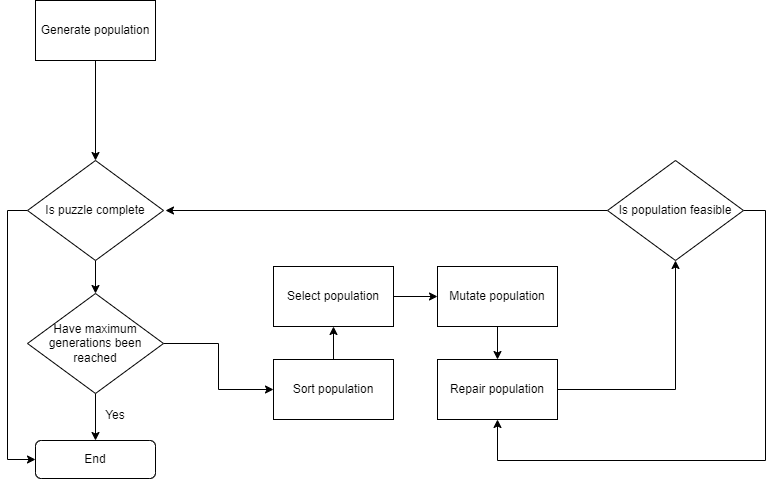
\includegraphics[height=5cm, width=8cm]{./Diagrams/hybridRepairFlowchart}
\end{figure}
\subsection{Approach for Multi-objective method}
The idea for the multi-objective method starts the same as the hybrid method, with generating the population of the puzzle. The next step is once again the same as for the hybrid repair method, the loop which ends if there are no violations and no empty spaces left in the puzzle or the maximum number of generations, and returns the solution if one was found. The next step is then mutating the puzzle, which in this algorithm, creates a copy set of children from the full population, mutates the children and then updates the fitness value of the children. The selection function now creates a new population, which is made from a combination of the two old populations, with the best between each parent and child pair being added to the new population.  

\begin{figure}[h]
	\caption{Flow diagram for Multi-objective method}
	\centering
	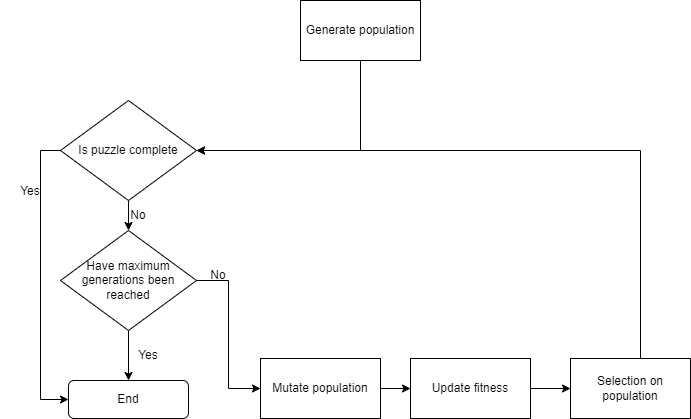
\includegraphics[height=5cm,width=8cm]{./Diagrams/multiobjectiveFlowchart}
\end{figure}
\newpage
\subsection{Experiment design}

The experiment, program will go over a set of 10 puzzles in a folder. For each puzzle in the dataset, it will loop through and solve each program storing the generations and time taken for each puzzle in an output file specific for that puzzle. Once all 30 runs of the solver have been done, the averages for the program can be calculated, the averages will not include failed attempts, as this will massively change the results and averages for successful runs. The failures will also be calculated and with the averages be added to a file specific to the puzzle size and difficulty. These results can then be processed using R, to create more meaningful data.
 
\subsection{Tools}
The programs used in this project are coded in Java 18, and are written in the IntelliJ IDEA IDE development environment. This is due to familiarity with the language and development environment. Within the development the use 3rd party library through Maven, JUnit was needed, to test individual features and functions of certain key methods, including ones listed in the requirements(see Chapter 3.1). GitHub was used as a version control tool and also used for project management , this was necessary as it allowed for a backup file system, which can be added to from different places, as well as providing a feature which can be used as a kanban board(mentioned in 1.4).
The statistical analysis needed for the experiments use the programming language R to perform the tests and produce graphs based on the data produced. texStudio and LaTeX were used in the creation of documentation providing a way to structure and document the final report for the project. The diagrams used in the documentation, were created using the tool draw.io, created diagrams visually explaining concepts, flowcharts used to show the basic outline of the program and class diagrams detailing each part of the project. 

\end{document}